\documentclass[conference]{IEEEtran}

\IEEEoverridecommandlockouts
\usepackage{cite}
\usepackage{amsmath,amssymb,amsfonts}
\usepackage{algorithmic}
\usepackage{graphicx}
\usepackage{textcomp}
\usepackage{xcolor}
\usepackage{fancyhdr}
\usepackage{lipsum}

\def\BibTeX{{\rm B\kern-.05em{\sc i\kern-.025em b}\kern-.08em
    T\kern-.1667em\lower.7ex\hbox{E}\kern-.125emX}}
    
\fancypagestyle{firstpagefooter}{%
  \fancyhf{}
  \renewcommand\headrulewidth{0pt}
  \fancyfoot[R]{IOT Challenges: Functional Safety, Hamm-Lippstadt Hochschule}
}

\pagestyle{empty}

\bibliographystyle{IEEEtran}

\begin{document}
\title{IOT Challenges: Functional Safety}

\author{\IEEEauthorblockN{Vytaras Juraska}
\IEEEauthorblockA{\textit{Electronics Engineering (7\textsuperscript{th} Semester)} \\
\textit{Hamm-Lippstadt Hochschule}\\
Lippstadt, Germany \\
vytaras.juraska@stud.hshl.de}
}

\maketitle

\begin{abstract}
in this paper main focus is emphasizing the importance of functional safety in the field of Internet Of Things (IOT), while also analyzing the today's standardised requirements, which each IOT device has to follow.
\end{abstract}

\thispagestyle{firstpagefooter}

\section{Introduction to Internet of Things (IOT)}

Quick introduction about the field itself

\subsection{General Applications of IOT}

Consumer applications, industrial applications (robustness, security, functional safety).

\section{Introduction to Functional Safety}
Short introduction to Functional Safety of IOT (FuSa for short). Maybe also a quick history part, of how it developed.

\section{Categories of Functional Safety}
What kind of FuSa categories are there, and how are they defined. Rely on the Reference \cite{robinson_living_2019}
\subsection{Machinery Safety Functions}

\begin{figure}[htbp]
\centerline{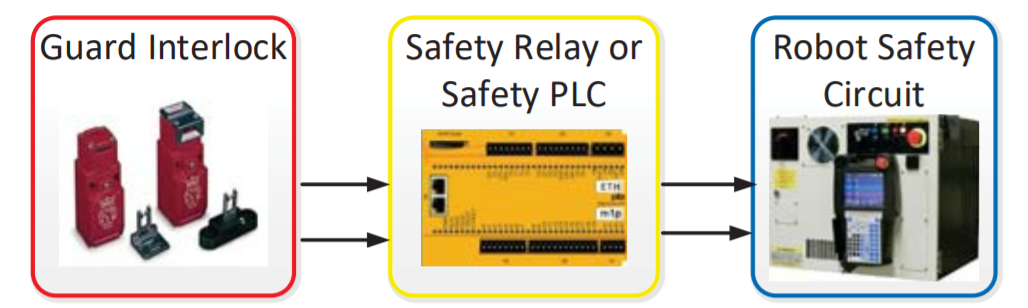
\includegraphics[scale=.33]{Machinery_FuSa.png}}
\caption{Safety block functions in machinery applications \cite{robinson_living_2019}}
\label{timeline}
\end{figure}

\subsection{Safety Integrity Level}

another category of FuSa, upon which I have to expand \cite{robinson_living_2019}

\section{Background of FuSa}

Which standards are important, general background.

\section{Example Issues and Unique Solutions}

Some examples of how IOT Functionality can go wrong and what was or might be done to avoid the problems. Rely on the Reference \cite{robinson_living_2019}

One of the examples could be Medical IOT System (Reference \cite{hayakawa_proposal_2018}).

\begin{figure}[htbp]
\centerline{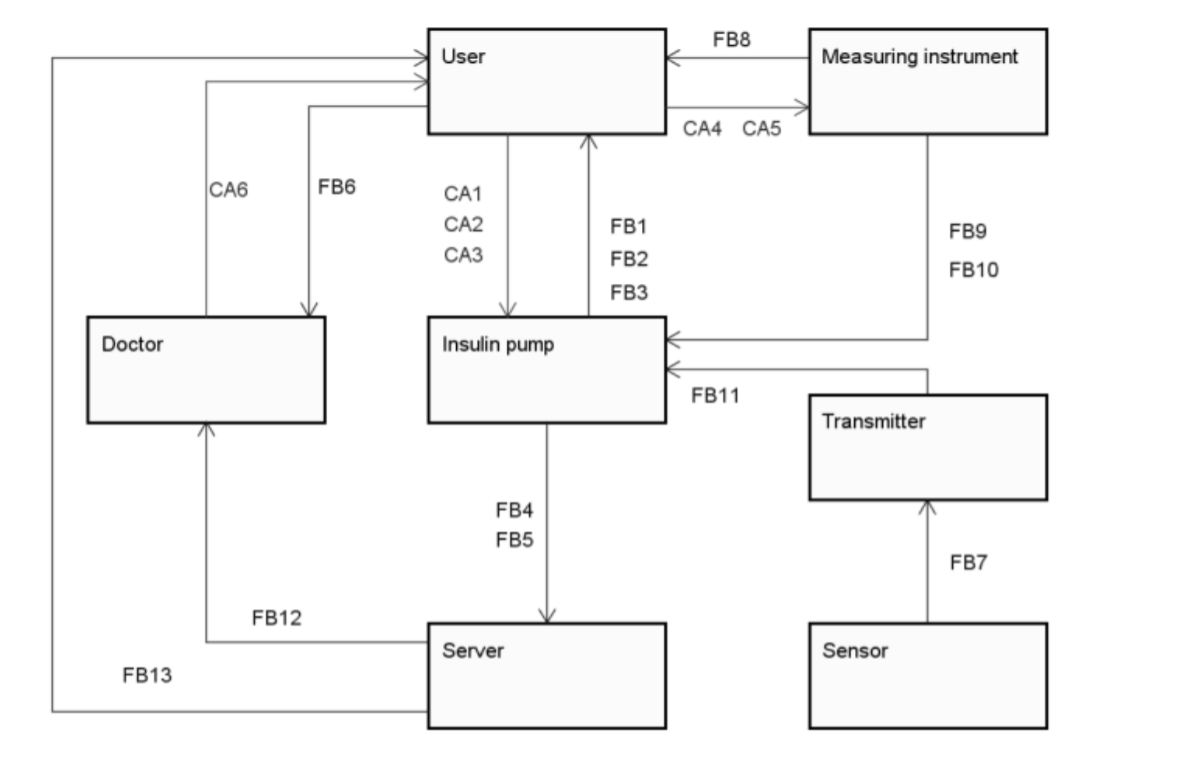
\includegraphics[scale=.33]{Medical_IOT.png}}
\caption{Example control structure in IOT application to medical field \cite{hayakawa_proposal_2018}}
\label{timeline}
\end{figure}

\section{Standardised Requirements}

\subsection{IEC 61508}

Rely on the document of References \cite{bell_introduction_nodate} and \cite{meany_functional_2017}.

\begin{figure}[htbp]
\centerline{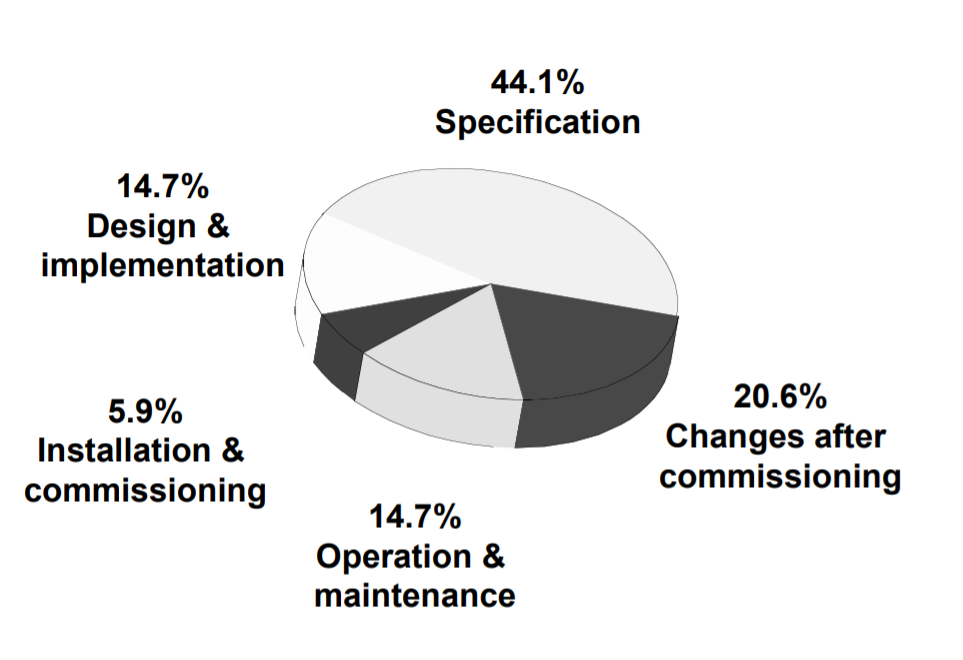
\includegraphics[scale=.33]{61508_SysFail.png}}
\caption{Main control system failure causes \cite{bell_introduction_nodate}}
\label{timeline}
\end{figure}

\subsection{ISO 13849}

Rely on the document of Reference \cite{meany_functional_2017} (also the document AN9025, which has the introduction to this standard).

\subsection{IEC 61784}

\section{Advantages of Functional Safety}

\section{Disadvantages of Functional Safety}

\section{Summary and Conclusion}

    Summary of paper and conclusion to the whole topic in one.

\section{Affidavit}
I, Vytaras Juraska, herewith declare that I have composed the present paper and work by our self and without use of any other than the cited sources and aids. Sentences or parts of sentences quoted literally are marked as such; other references with regard to the statement and scope are indicated by full details of the publications concerned. The paper and work in the same or similar form has not been submitted to any examination body and has not been published. This paper was not yet, even in part, used in another examination or as a course performance.

\bibliography{references}

\end{document}
